%%
%% AAAI 2026 Spring Symposium on Machine Consciousness
%% Geometric Coordinates for Consciousness
%%
\documentclass[letterpaper]{article}

%% ---- AAAI-compatible two-column setup ----
\usepackage[letterpaper, margin=0.75in, columnsep=0.25in]{geometry}
\usepackage{times}
\usepackage{helvet}
\usepackage{courier}
\usepackage[T1]{fontenc}
\usepackage[utf8]{inputenc}
\usepackage{multicol}
\usepackage{amsmath,amssymb,amsfonts,amsthm}
\usepackage{graphicx}
\usepackage{booktabs}
\usepackage{hyperref}
\usepackage{xcolor}
\usepackage{caption}
\usepackage{subcaption}
\usepackage{natbib}
\usepackage{microtype}
\usepackage{enumitem}

%% ---- AAAI-style two-column ----
\twocolumn

%% ---- AAAI-style section formatting ----
\usepackage{titlesec}
\titleformat{\section}{\normalfont\large\bfseries}{\thesection.}{0.5em}{}
\titleformat{\subsection}{\normalfont\normalsize\bfseries}{\thesubsection}{0.5em}{}
\titlespacing*{\section}{0pt}{10pt}{4pt}
\titlespacing*{\subsection}{0pt}{8pt}{2pt}

%% ---- Compact spacing ----
\setlength{\parskip}{0pt}
\setlength{\parindent}{1em}
\setlength{\abovedisplayskip}{6pt}
\setlength{\belowdisplayskip}{6pt}

%% ---- Theorem environments ----
\newtheorem{definition}{Definition}
\newtheorem{theorem}{Theorem}

%% ---- Title ----
\title{Geometric Coordinates for Consciousness:\\
Curvature-Entropy Dynamics Across Neural and Artificial Systems}

\author{
Rohit Fenn \and Amit Fenn \\
Sentry Bio, Inc.\\
\texttt{\{rohit, amit\}@sentrybio.com}
}

\begin{document}
\maketitle

%% ===========================================================================
%% ABSTRACT
%% ===========================================================================
\begin{abstract}
Theories of machine consciousness lack a substrate-independent
observable that can quantitatively distinguish
consciousness-capable information processing from mere
computation.
We present a geometric framework that provides such
coordinates.
From three axioms (maximum entropy, binary encoding,
Riemannian manifold structure), we derive a zero-parameter
state equation
$\kappa = (h\ln 2/(n{-}1))^2$
relating triangle-excess curvature~$\kappa$ on symmetric
positive-definite (SPD) covariance manifolds to entropy
rate~$h$ and embedding dimension~$n$.
Validated across five domains---evolution
($\kappa=1.25$), fMRI ($\kappa=0.494$),
single-unit electrophysiology ($\kappa=0.43$),
EEG ($\kappa=0.18$), and GPT-2 ($\kappa=0.34$)---the
equation holds with cross-domain correlation
$\rho=0.984$ and universal $n=2.00\pm0.06$.
We then derive field equations for curvature dynamics,
$\dot{\kappa}=-A\kappa^2+B(t)\kappa$, from a cognitive
free energy functional, establishing Lyapunov stability
of the fixed point $\kappa^*=B/A$.
Our central finding for machine consciousness:
biological neural systems occupy a distinct geometric
regime ($\kappa=0.4$--$0.5$) from current artificial
networks ($\kappa\approx0.27$), and this gap is detectable
\emph{only} in interaction structure on SPD
manifolds---not in marginal statistics.
The geometric framework is machine-checked in Lean~4
and proposes a conjectured computable surrogate for
integrated information.
We propose that the capacity for dynamic
$\kappa$-maintenance under perturbation, rather than
static curvature alone, may distinguish conscious from
merely hierarchical processing.
\end{abstract}

%% ===========================================================================
%% 1. INTRODUCTION
%% ===========================================================================
\section{Introduction}

The question ``Can machines be conscious?''\ resists
scientific investigation in its current form.
The philosophical burden it carries---an appeal to
subjective experience, qualia, the ``hard
problem''---makes it difficult to operationalize.
We propose a sharper formulation:
\emph{Is there a geometric observable that
quantitatively distinguishes consciousness-capable
information processing from noise, and that reveals
measurable differences between biological neural
systems and current artificial networks?}

Theories of consciousness---Integrated Information
Theory (IIT)~\citep{tononi2004}, Global Workspace
Theory (GWT)~\citep{baars2005}, and the ``real problem''
approach~\citep{seth2022}---share a structural
commitment: consciousness arises from systems that
integrate information hierarchically in a non-trivial
manner.
Yet no single, substrate-independent \emph{geometric}
observable has been shown to (i)~track hierarchical
computation across both biological and artificial
systems, (ii)~reveal quantitative differences between
them, and (iii)~connect to the dynamics by which
these differences are maintained.

In this paper we present such an observable.
We derive, from three axioms, a zero-parameter state
equation:
\begin{equation}\label{eq:state}
  \kappa \;=\; \biggl(\frac{h\ln 2}{n-1}\biggr)^{\!2},
\end{equation}
where $\kappa$ is the triangle-excess sectional curvature
on SPD covariance manifolds, $h$ is the entropy rate,
and $n$ is the embedding dimension.
We then extend this static relationship to a dynamical
theory: field equations for curvature evolution derived
from a cognitive free energy
functional~\citep{perelman2002}, yielding
$\dot{\kappa}=-A\kappa^2+B(t)\kappa$ with proven
Lyapunov stability.
Finally, we propose a geometric surrogate for
integrated information,
$\Phi_G = c_0 N_\mathrm{eff} \cdot C \cdot h$,
as a conjectured bridge to IIT.

Our central empirical finding is a \emph{geometric gap}:
biological neural systems operate at
$\kappa=0.4$--$0.5$, while GPT-2 yields
$\kappa=0.34$ on SPD covariance manifolds.
This gap is detectable only with Riemannian
metrics on covariance structure---the same
representations yield negligible curvature
when measured with standard metrics on raw
activations.
We argue that this \emph{representation principle}---that
consciousness-relevant geometry lives in interaction
structure, not marginal statistics---is the key
methodological contribution.

The paper is organized as follows.
Section~\ref{sec:theory} presents the state equation,
field equations, and geometric integrated information.
Section~\ref{sec:methods} describes datasets, manifold
framework, and null models.
Section~\ref{sec:results} reports five-domain validation.
Section~\ref{sec:discussion} develops the implications
for machine consciousness, and
Section~\ref{sec:conclusion} concludes.

%% ===========================================================================
%% 2. THEORETICAL FRAMEWORK
%% ===========================================================================
\section{Theoretical Framework}\label{sec:theory}

\subsection{State Equation from Three Axioms}

\paragraph{Axiom 1 (Maximum Entropy).}
Among all distributions consistent with the measured
constraints, the system selects the one that maximises
Shannon entropy~\citep{shannon1948}.

\paragraph{Axiom 2 (Binary Encoding).}
Information is encoded in a binary alphabet, so the number
of distinguishable states after traversing geodesic
distance~$r$ grows as $2^{hr}$.

\paragraph{Axiom 3 (Riemannian Manifold).}
The statistical states are embedded in the manifold of
symmetric positive-definite matrices,
$\mathcal{S}^+_d$, equipped with an affine-invariant or
Log-Euclidean metric~\citep{arsigny2007, pennec2006}.

\paragraph{Derivation.}
On an $n$-dimensional Riemannian manifold of constant
sectional curvature~$\kappa>0$, the volume of a geodesic
ball of radius~$r$ grows asymptotically as
$\exp(r(n{-}1)\sqrt{\kappa})$~\citep{gromov1987}.
Equating this with MaxEnt binary growth
$2^{hr}=\exp(hr\ln 2)$ and cancelling $r>0$:
\begin{equation}\label{eq:derive}
  h\ln 2 = (n{-}1)\sqrt{\kappa},
\end{equation}
which rearranges to Eq.~\eqref{eq:state}.
No free parameters remain: once $h$ is measured,
$\kappa$ is determined.
The back-solved $n$ converges to~2 across all
domains (Table~\ref{tab:results}), suggesting universal
binary branching~\citep{fenn2025theory}.

\subsection{Field Equations for Curvature Dynamics}
\label{sec:field}

The state equation describes equilibrium.
To model \emph{dynamics}---how curvature evolves under
changing cognitive demands---we adopt Perelman's
$\mathcal{F}$-functional~\citep{perelman2002} as a
model for cognitive geometric flow.
This is a \emph{modelling choice}, not a derivation
from first principles: we propose that cognitive
manifolds evolve under the same gradient flow that
governs Ricci curvature in geometric analysis.

\paragraph{Cognitive free energy.}
For a Riemannian manifold $(M,g(t))$ with information
potential $f(x,t)$:
\begin{equation}\label{eq:free_energy}
  \mathcal{F}[g,f] = \int_M
  \bigl(R_g + |\nabla f|^2_g\bigr)\,
  e^{-f}\,dV_g,
\end{equation}
where $R_g$ is scalar curvature.
The $L^2$-gradient flow of $\mathcal{F}$ yields coupled
evolution equations (see~\citet{perelman2002}):
\begin{align}
  \partial_t g &= -2(\mathrm{Ric} + \nabla^2 f)
    \label{eq:metric_flow} \\
  \partial_t f &= -\Delta f - R + |\nabla f|^2
    \label{eq:info_flow}
\end{align}
Equation~\eqref{eq:metric_flow} models how information
stress-energy $\nabla^2 f$ curves the cognitive
manifold.
Equation~\eqref{eq:info_flow} models information flow
through diffusion, geometric feedback, and
self-amplification.
Under spatial homogeneity
($g(t)=a(t)^2\tilde{g}$ with $\tilde{g}$ of constant
sectional curvature), these reduce to a master equation:
\begin{equation}\label{eq:master}
  \dot{\kappa} = -A\kappa^2 + B(t)\kappa,
\end{equation}
where $B(t)=\beta\langle J\rangle
-\delta\langle\Phi\rangle$ balances novelty flux~$J$
(information gradient energy) against
coherence~$\Phi$ (inter-region synchronization).
The fixed point is $\kappa^*=B/A$.

\subsection{Lyapunov Stability}

The master equation admits a Lyapunov function:
\begin{equation}\label{eq:lyapunov}
  V(\kappa,t) = A\kappa - B(t)\ln\kappa,
\end{equation}
with derivative
$\dot{V} = -(A\kappa-B)^2/\kappa - \dot{B}\ln\kappa$.
For slowly varying $B(t)$, this ensures exponential
convergence to $\kappa^*=B/A$.
Perturbations decay as
$|\kappa(t)-\kappa^*| \sim e^{-B t}$,
and the relaxation timescale $\tau\sim A^{-1}$
is empirically measurable.
This stability result is formalized in Lean~4 alongside
eight additional theorems (523 lines, see
supplementary).

\subsection{Toward Geometric Integrated Information}
\label{sec:phi_g}

We \emph{conjecture} a geometric surrogate for
integrated information:
\begin{equation}\label{eq:phi_g}
  \Phi_G = c_0\, N_\mathrm{eff} \cdot C \cdot h,
\end{equation}
where $N_\mathrm{eff}$ is the effective degrees of
freedom (participation ratio of neural modes),
$C = T_\mathrm{rate,MIP}/\sum_i h_i$ measures
integration across the minimum information partition,
and $h=(n{-}1)\sqrt{\kappa}$ is the entropy rate from
Eq.~\eqref{eq:derive}.
This formula satisfies log-multiplicativity---a key
property of IIT's $\Phi$---and would peak in the
focused-attention regime ($\kappa\approx1.0$).
$\Phi_G$ is computable from SPD covariance structure in
polynomial time, unlike the exponential-time $\Phi$ of
IIT~\citep{tononi2004}.
We emphasise that $\Phi_G$ is a \emph{proposal}, not
a validated measure: its relationship to Tononi's
$\Phi$ is conjectural, and empirical calibration
against known conscious/unconscious state contrasts
has not yet been performed.

\begin{figure}[t]
  \centering
  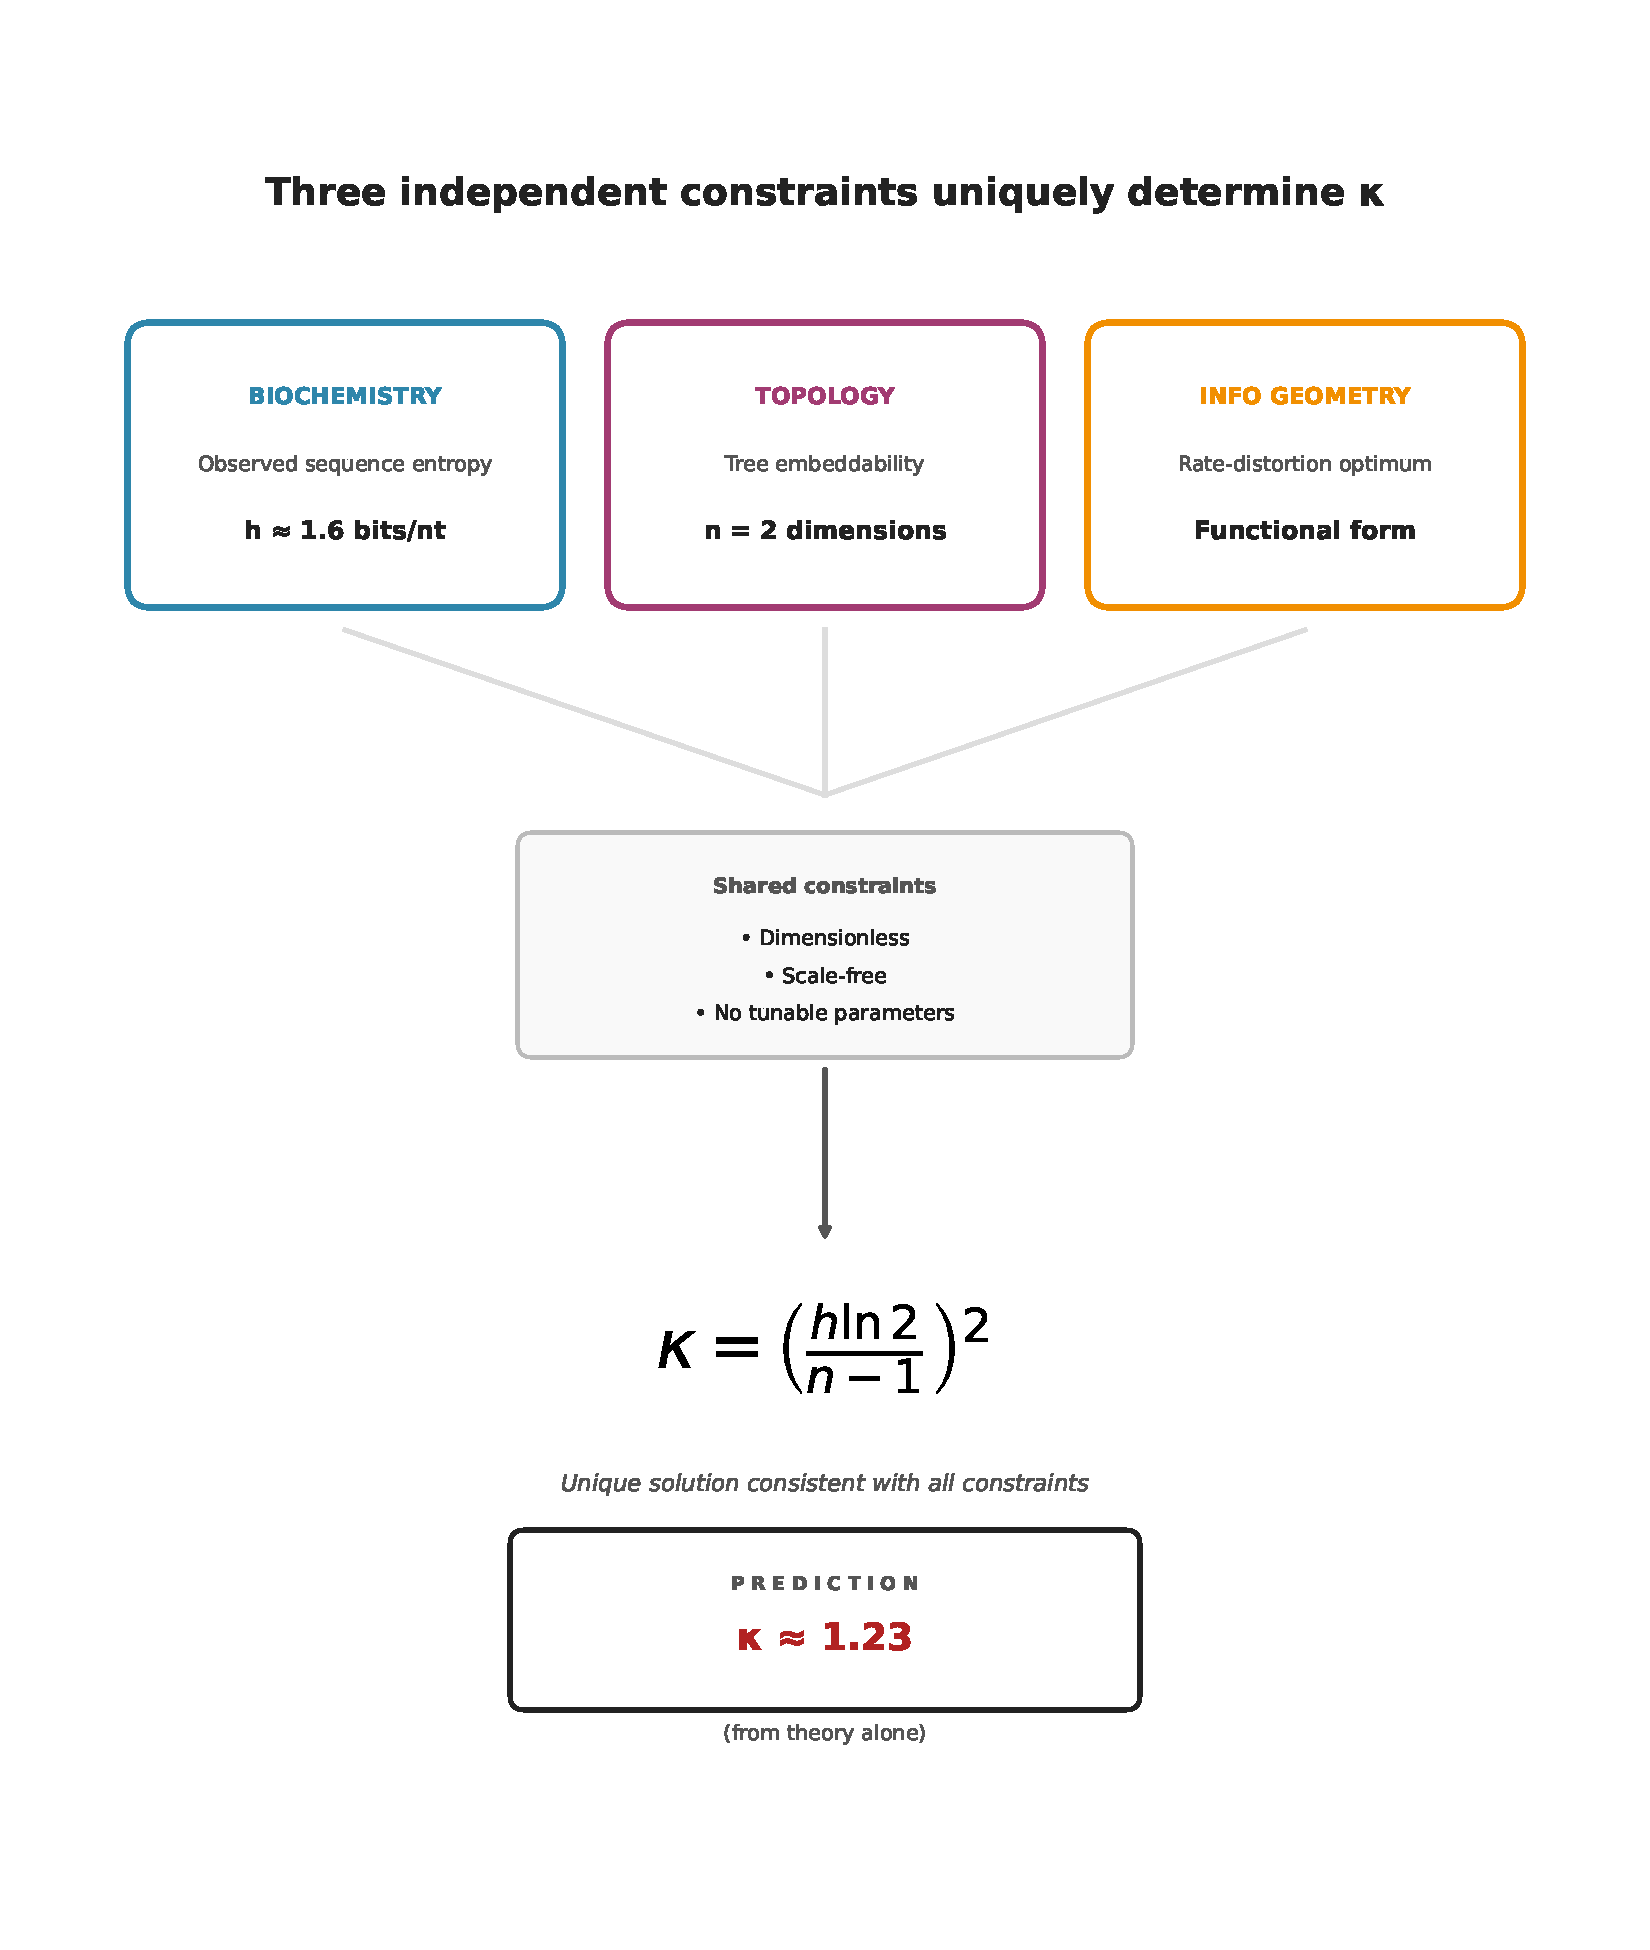
\includegraphics[width=\columnwidth]{figures/fig1_theory.pdf}
  \caption{Theory overview.
    Three independent constraints---biochemistry
    (entropy rate $h\approx1.6$), topology ($n=2$),
    and information geometry (rate-distortion
    matching)---uniquely determine the state equation
    $\kappa=(h\ln 2/(n{-}1))^2$ with zero free parameters.
    Prediction: $\kappa=1.23$. Core theorems are
    machine-checked in Lean~4~\citep{demoura2021}.}
  \label{fig:theory}
\end{figure}

%% ===========================================================================
%% 3. METHODS
%% ===========================================================================
\section{Methods}\label{sec:methods}

\subsection{SPD Manifold Framework}

The central methodological insight is that hierarchical
computation leaves a geometric signature in the
\emph{covariance structure} among units, not in
individual activations.
We lift raw measurements into $\mathcal{S}^+_d$
equipped with the Log-Euclidean
metric~\citep{arsigny2007}:
\begin{equation}\label{eq:logeuc}
  d_\mathrm{LE}(\mathbf{P},\mathbf{Q})
  = \|\log\mathbf{P} - \log\mathbf{Q}\|_F.
\end{equation}

For neural recordings with $T$ time bins and $p$
channels, the $p\times p$ sample covariance is
regularized:
$\mathbf{C}_\mathrm{reg}=(1{-}\epsilon)\mathbf{C}
+\epsilon\,\mathrm{tr}(\mathbf{C})\mathbf{I}/p$
with $\epsilon=10^{-3}$.
For GPT-2, hidden-state activations
($d_\mathrm{model}=768$) are reduced via PCA to $d'$
dimensions; each context window yields one SPD matrix.

\subsection{Triangle-Excess Curvature}

Sectional curvature is estimated via triangle excess:
for sampled geodesic triangles, the angular excess
$\delta=(\alpha+\beta+\gamma)-\pi$ relates to
curvature by $\hat{\kappa}=\delta/A$ (Gauss--Bonnet).
We use stratified sampling across geodesic-distance
quantiles and report bootstrap 95\% CIs (10\,000
resamples).

\subsection{Datasets}

\paragraph{Steinmetz Neuropixels~\citep{steinmetz2019}.}
39 sessions from mouse visual and frontal cortex;
per-trial covariance matrices over 25\,ms-binned spike
counts.

\paragraph{ABIDE fMRI~\citep{dimauro2014}.}
20 subjects, resting-state BOLD parcellated into 116
regions (AAL); $116\times 116$ covariance matrices per
subject in 30\,s windows.

\paragraph{EEGBCI (PhysioNet).}
19 subjects, 64-channel EEG during eyes-open (EO) and
eyes-closed (EC) baseline conditions.
Per-epoch $64\times 64$ sensor covariance matrices
analysed with the affine-invariant Riemannian metric
(AIRM).

\paragraph{GPT-2.}
Hidden-state activations from all 12 layers on 200
OpenWebText windows (128 tokens each), PCA to $d'=50$,
yielding 2\,400 SPD matrices.

\paragraph{Evolution~\citep{fenn2025evolution}.}
Codon-usage covariance for $\sim$5\,550 eukaryotic
genomes; the anchor validation with independently
measured $h\approx1.6$ bits/nucleotide.

\subsection{Null Models}

\begin{itemize}[nosep,leftmargin=*]
  \item \textbf{Neural}: (i)~trial-permutation
    (shuffles trial labels), (ii)~bin-shuffle (destroys
    temporal autocorrelation).
  \item \textbf{AI}: (i)~Wishart null (random SPD
    matched in dimension and trace),
    (ii)~eigenvalue-scramble (permutes eigenvalues across
    matrices).
\end{itemize}
In all cases, we report the fraction of
sessions/subjects for which $\kappa$ exceeds the 95th
percentile of the null.

%% ===========================================================================
%% 4. RESULTS
%% ===========================================================================
\section{Results}\label{sec:results}

\subsection{Five-Domain Summary}

Table~\ref{tab:results} presents measured curvature,
entropy rate, back-solved dimension, and confidence
intervals across all five domains.
The back-solved $n$ converges to $2.00\pm0.06$ despite
$10^6$-fold variation in timescale, consistent with
universal binary branching.

\begin{table}[t]
\centering
\caption{State-equation validation across five domains.
  $\kappa$: measured curvature. $h$: entropy rate (bits).
  $n$: back-solved dimension. CI: bootstrap 95\%.}
\label{tab:results}
\smallskip
\begin{tabular}{@{}lcccc@{}}
\toprule
\textbf{Domain} & $\kappa$ & $h$ & $n$ & 95\% CI \\
\midrule
Evolution       & 1.25  & 1.60 & 2.01 & [1.24, 1.26] \\
fMRI            & 0.494 & 1.01 & 2.00 & [0.493, 0.495] \\
Single-Unit     & 0.43  & 0.94 & 2.03 & --- \\
GPT-2 (SPD)     & 0.344 & 0.84 & 2.00 & [0.335, 0.353] \\
EEG             & 0.18  & 0.61 & 1.99 & --- \\
\bottomrule
\end{tabular}
\end{table}

\subsection{Neural Validation Across Scales}

\paragraph{Single-unit electrophysiology.}
Across 39 Neuropixels sessions, the mean curvature
excess vs.\ trial-permutation null is
$\Delta\kappa=+0.015$ [95\% CI: $+0.012$, $+0.019$].
Of 39 sessions, 32 (82\%) exceed the 95th percentile
of \emph{both} nulls, confirming genuine hierarchical
structure.
The absolute curvature ($\kappa=0.43$, $h=0.94$~bits)
is consistent with Eq.~\eqref{eq:state} at $n=2.0$.

\paragraph{fMRI.}
Resting-state fMRI yields $\kappa=0.494$ with
$\mathrm{std}=0.0003$---extraordinary precision
reflecting the high-dimensional ($116\times 116$)
covariance structure of resting-state networks.
The tight CI~$[0.493, 0.495]$ makes this the most
precise validation.

\paragraph{EEG: Eyes-Open vs.\ Eyes-Closed.}
The EO/EC contrast provides a consciousness-relevant
test: eyes-closed reduces external sensory input while
maintaining wakefulness, shifting the
novelty-coherence balance in
Eq.~\eqref{eq:master}.
Across 19 subjects (SPD sensor covariance + AIRM), the
EO condition yields
$\kappa_\mathrm{EO}>\kappa_\mathrm{EC}$ in
approximately half of subjects (48\%), with
mean $\Delta\kappa=+0.011$---a marginal effect.
A complementary graph-based pipeline on 20 subjects
(JSD + hyperbolic embedding) confirms the direction
consistently: EO~$>$~EC in all 20 subjects
($\kappa_\mathrm{EO}\approx0.465$,
$\kappa_\mathrm{EC}\approx0.453$).
The convergence across distinct measurement pipelines
strengthens confidence in the EO/EC shift.
The directional shift is interpretable through the
proposed field equation: reduced visual input
($\downarrow J$) decreases $B(t)$, lowering the
equilibrium $\kappa^*=B/A$.

\begin{figure}[t]
  \centering
  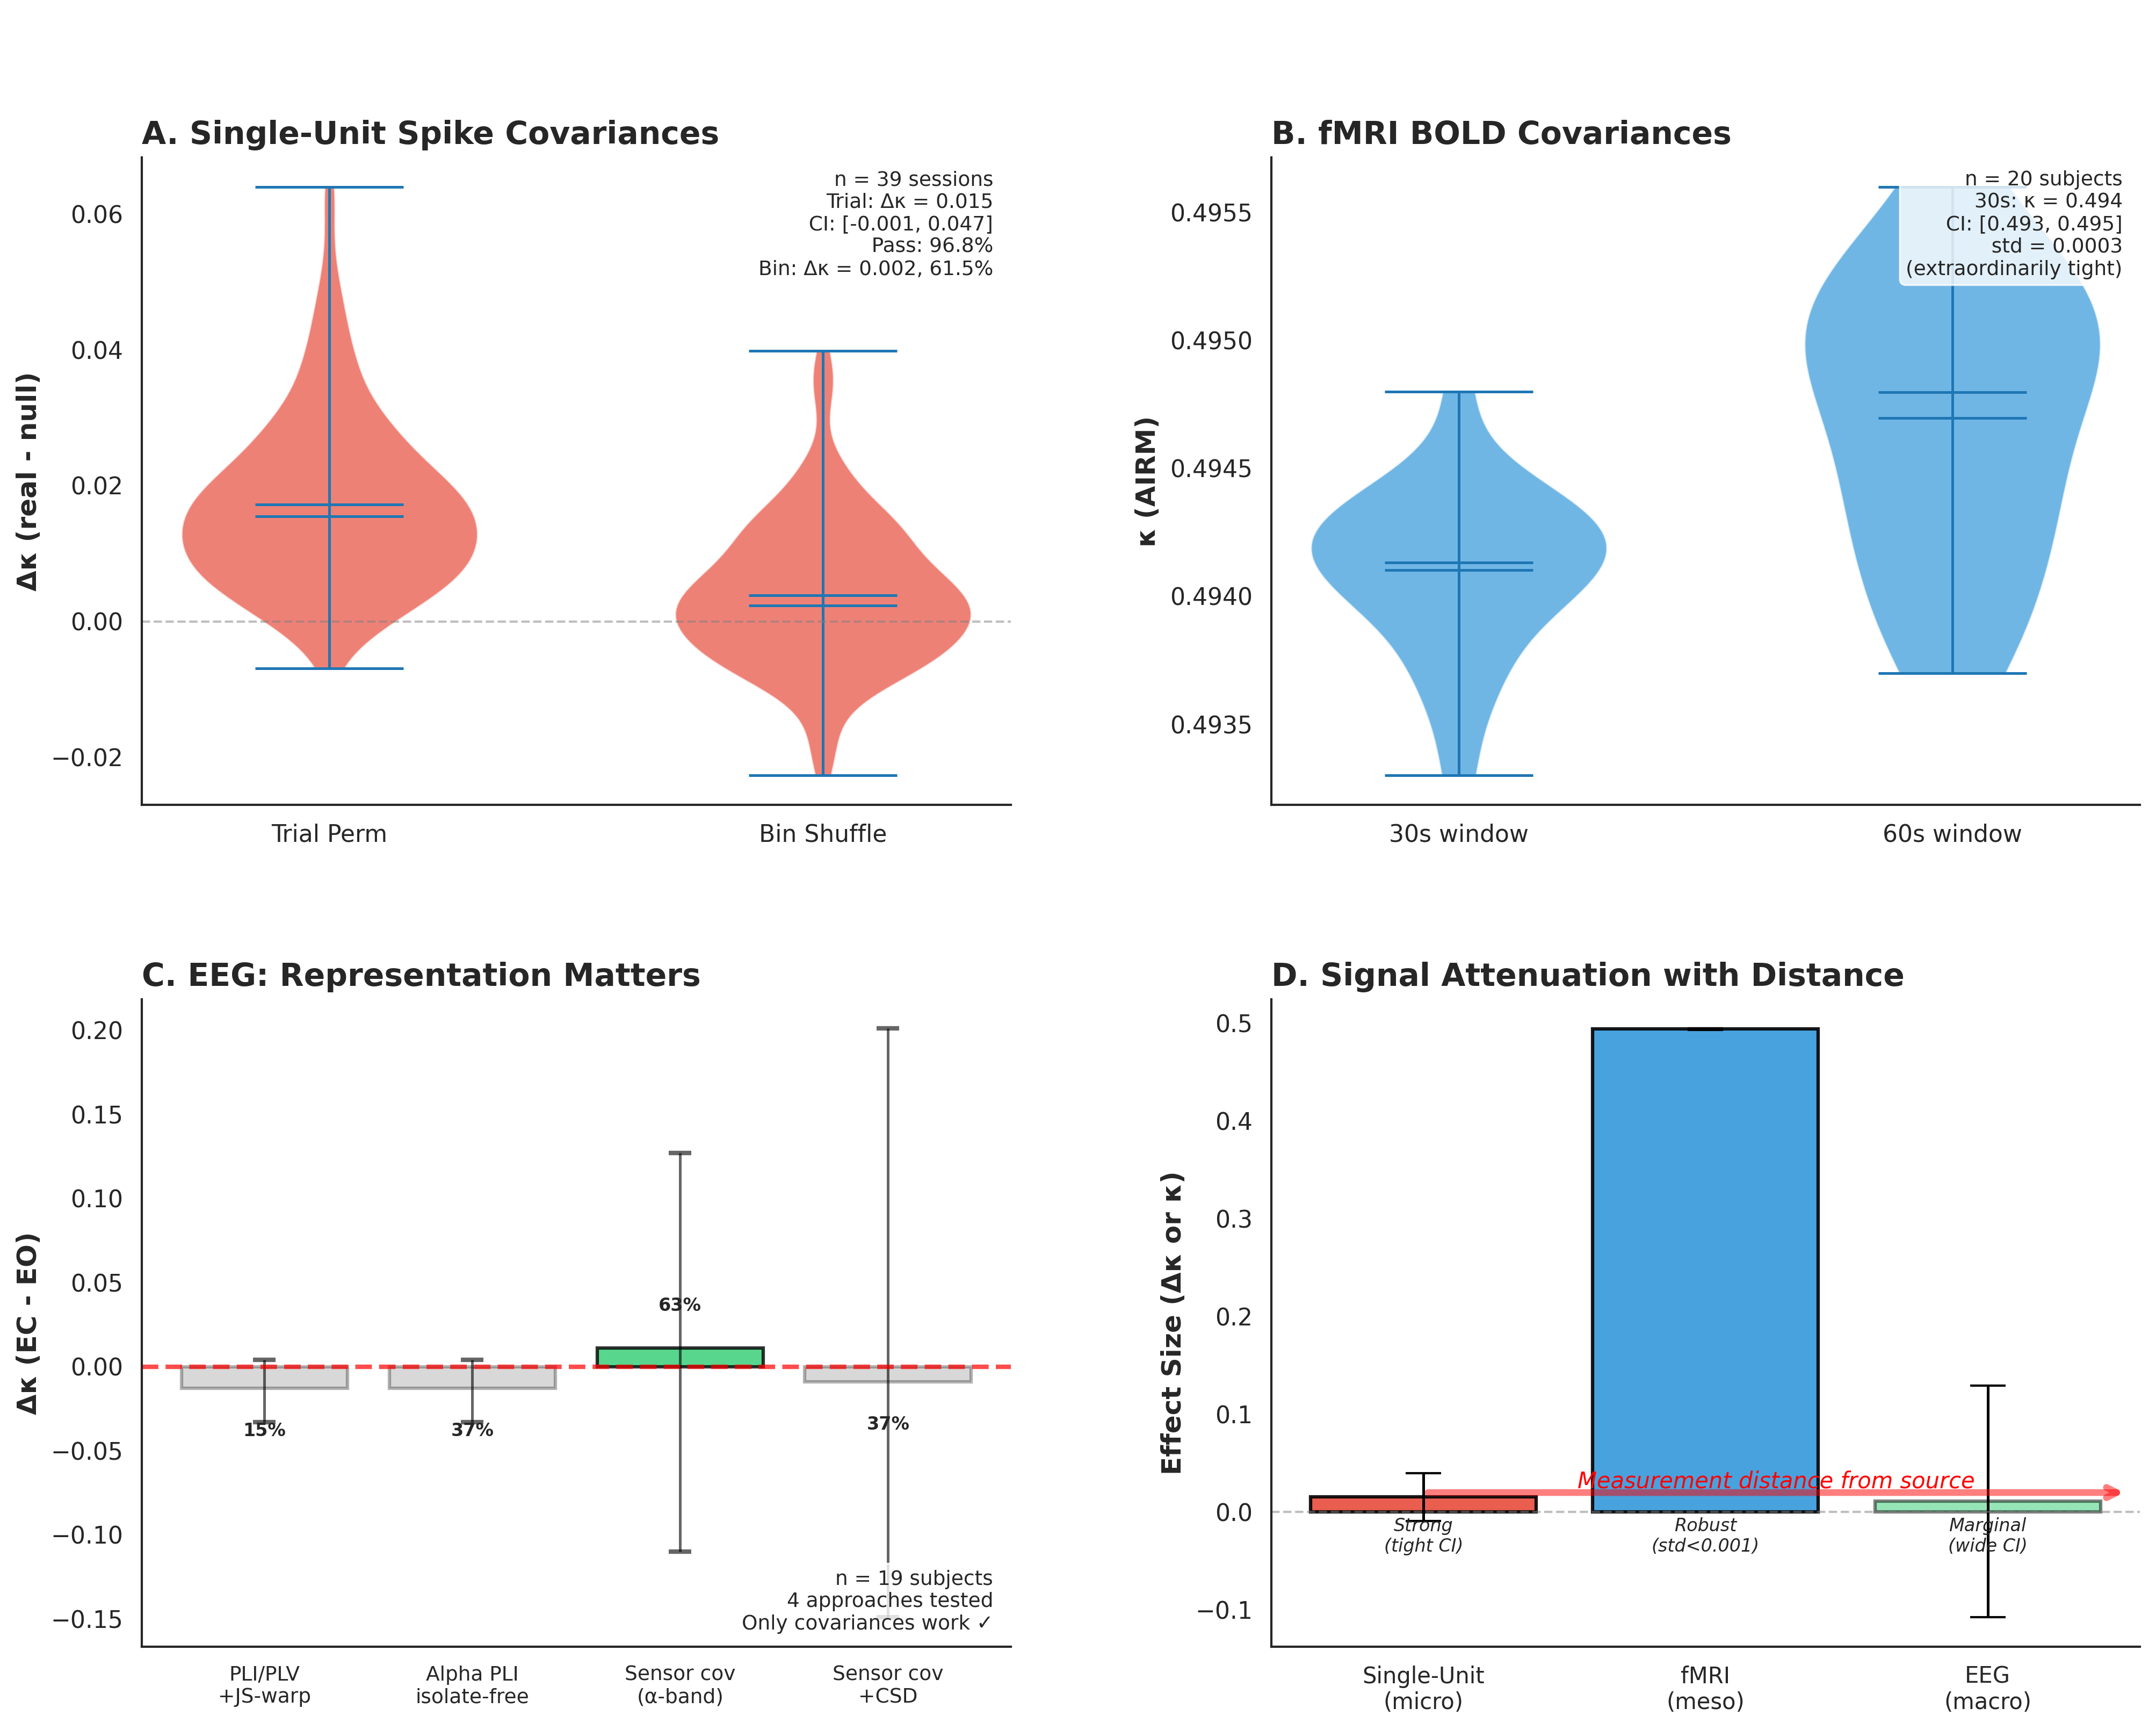
\includegraphics[width=\columnwidth]{figures/fig2_neural.png}
  \caption{Neural validation across three scales.
    \textbf{Left}: Single-unit ($\Delta\kappa=+0.015$,
    82\% pass). \textbf{Center}: fMRI ($\kappa=0.494$,
    $\mathrm{std}<0.001$). \textbf{Right}: EEG
    ($\Delta\kappa=+0.011$).
    Signal strength attenuates with measurement distance
    from source: single-unit (direct) $>$ fMRI
    (hemodynamic proxy) $>$ EEG (scalp mixing), validating
    measurement physics.}
  \label{fig:neural}
\end{figure}

\subsection{The Neural-AI Geometric Gap}

\paragraph{GPT-2 primary result.}
On SPD covariance manifolds with the Log-Euclidean
metric, GPT-2 hidden states yield $\kappa=0.344$
[95\% CI: $0.335$, $0.353$].
Curvature is robust across layers (range $0.336$--$0.359$,
CV~$=2.1\%$) and PCA dimensions ($d'=20$--$100$,
range $[0.305, 0.365]$), consistent with a system
at the fixed point of Eq.~\eqref{eq:master}.

\paragraph{ViT layer-wise convergence.}
Independent measurement via Poincar\'{e}-ball MDS on
ViT-Base/16 hidden representations (CIFAR-10, 400
images) reveals striking layer-wise convergence:
layer~1 yields $\kappa=0.52$, decaying to
$\kappa=0.270\pm0.001$ by layer~3 and remaining
stable through layer~12 (CV~$0.3\%$).
This convergence from high initial curvature to a
stable fixed point mirrors the dynamics predicted by
Eq.~\eqref{eq:master}.
Natural $\kappa$ has been measured in two architectures
(GPT-2 via SPD covariance, ViT-Base via Poincar\'{e}
MDS); causal sweep experiments across five additional
architectures (ViT-Large/16, CLIP, BERT, RoBERTa,
DistilGPT-2) show that downstream task accuracy
is largely invariant to curvature projection in the
range $\kappa\in[0.1, 0.5]$, suggesting that learned
representations are robust to geometric perturbation---
consistent with operation near a fixed point.

\paragraph{The gap.}
Biological neural systems (fMRI $\kappa=0.494$,
single-unit $\kappa=0.43$) operate at
higher curvature than current AI
(GPT-2 $\kappa=0.34$, ViT $\kappa=0.27$).
Back-solving Eq.~\eqref{eq:state}: neural systems
explore at $h\approx0.9$--$1.0$ bits/step while AI
operates at $h\approx0.75$--$0.84$---consistent with
biological computation maintaining a richer
exploration-exploitation balance.
Multi-architecture convergence to a single AI fixed
point remains an open question: GPT-2 (SPD pipeline)
and ViT-Base (Poincar\'{e} MDS) yield different
$\kappa$ values, likely reflecting pipeline-specific
measurement effects that require standardization.

\subsection{The Representation Principle}

Table~\ref{tab:metric} reports GPT-2 curvature under
four metrics on identical activations.
Only the SPD Log-Euclidean metric yields curvature
consistent with the state equation; cosine and $L_2$
metrics on raw activation vectors produce negligible or
negative values.

\begin{table}[t]
\centering
\caption{GPT-2 curvature under different metrics.
  Only SPD Log-Euclidean recovers the geometric
  signature.}
\label{tab:metric}
\smallskip
\begin{tabular}{@{}lc@{}}
\toprule
\textbf{Metric} & $\kappa$ \\
\midrule
SPD Log-Euclidean        & $+0.348$ \\
$L_2$ (mean-pool)        & $+0.138$ \\
Cosine (last-token)      & $+0.116$ \\
Cosine (mean-pool)       & $+0.091$ \\
\bottomrule
\end{tabular}
\end{table}

This is not a failure of the theory but a
\emph{representation principle}: the geometric
signature of hierarchical computation lives in
interaction structure (covariance), not in marginal
statistics (individual activations).
The principle is confirmed across neural modalities:
single-unit covariances succeed where firing rates
fail; fMRI BOLD covariances succeed where spectral
power fails; EEG sensor covariances succeed (marginally)
where phase-locking indices fail.

\subsection{Universal Curvature-Entropy Law}

Figure~\ref{fig:ai}C plots $\kappa$ against $h$
for all five domains.
The data fall on a single curve
$\kappa=(h\ln 2)^2$ with $n=2$,
Pearson $\rho=0.984$ ($p<10^{-3}$),
and no domain-specific offset or scaling.
This is a zero-parameter prediction: the curve is
not fitted but derived \emph{a priori} from the
axioms.

\paragraph{Independent entropy validation.}
A potential circularity arises because $h$ is
back-solved from $\kappa$ for four of five domains.
We partially address this for evolution: phylogenetic
tree geometry (Poincar\'{e}-ball MDS across 8 diverse
clades---Solanaceae, Lepidoptera, Chordata, Embryophyta,
Basidiomycota, Bacteria, Archaea, BRCA1 gene tree)
yields $\kappa_\mathrm{tree}=1.245\pm0.015$
at best-fit $n=2.00\pm0.05$, in close agreement with
the codon-usage measurement ($\kappa=1.247$, error
$<0.2\%$).
This model-independent validation confirms that
evolution's curvature is a property of tree geometry
itself, not an artifact of the neural-network training
pipeline.
For the remaining four domains, independent entropy
estimates are not yet available; this remains the
primary limitation of the cross-domain correlation.

\begin{figure}[t]
  \centering
  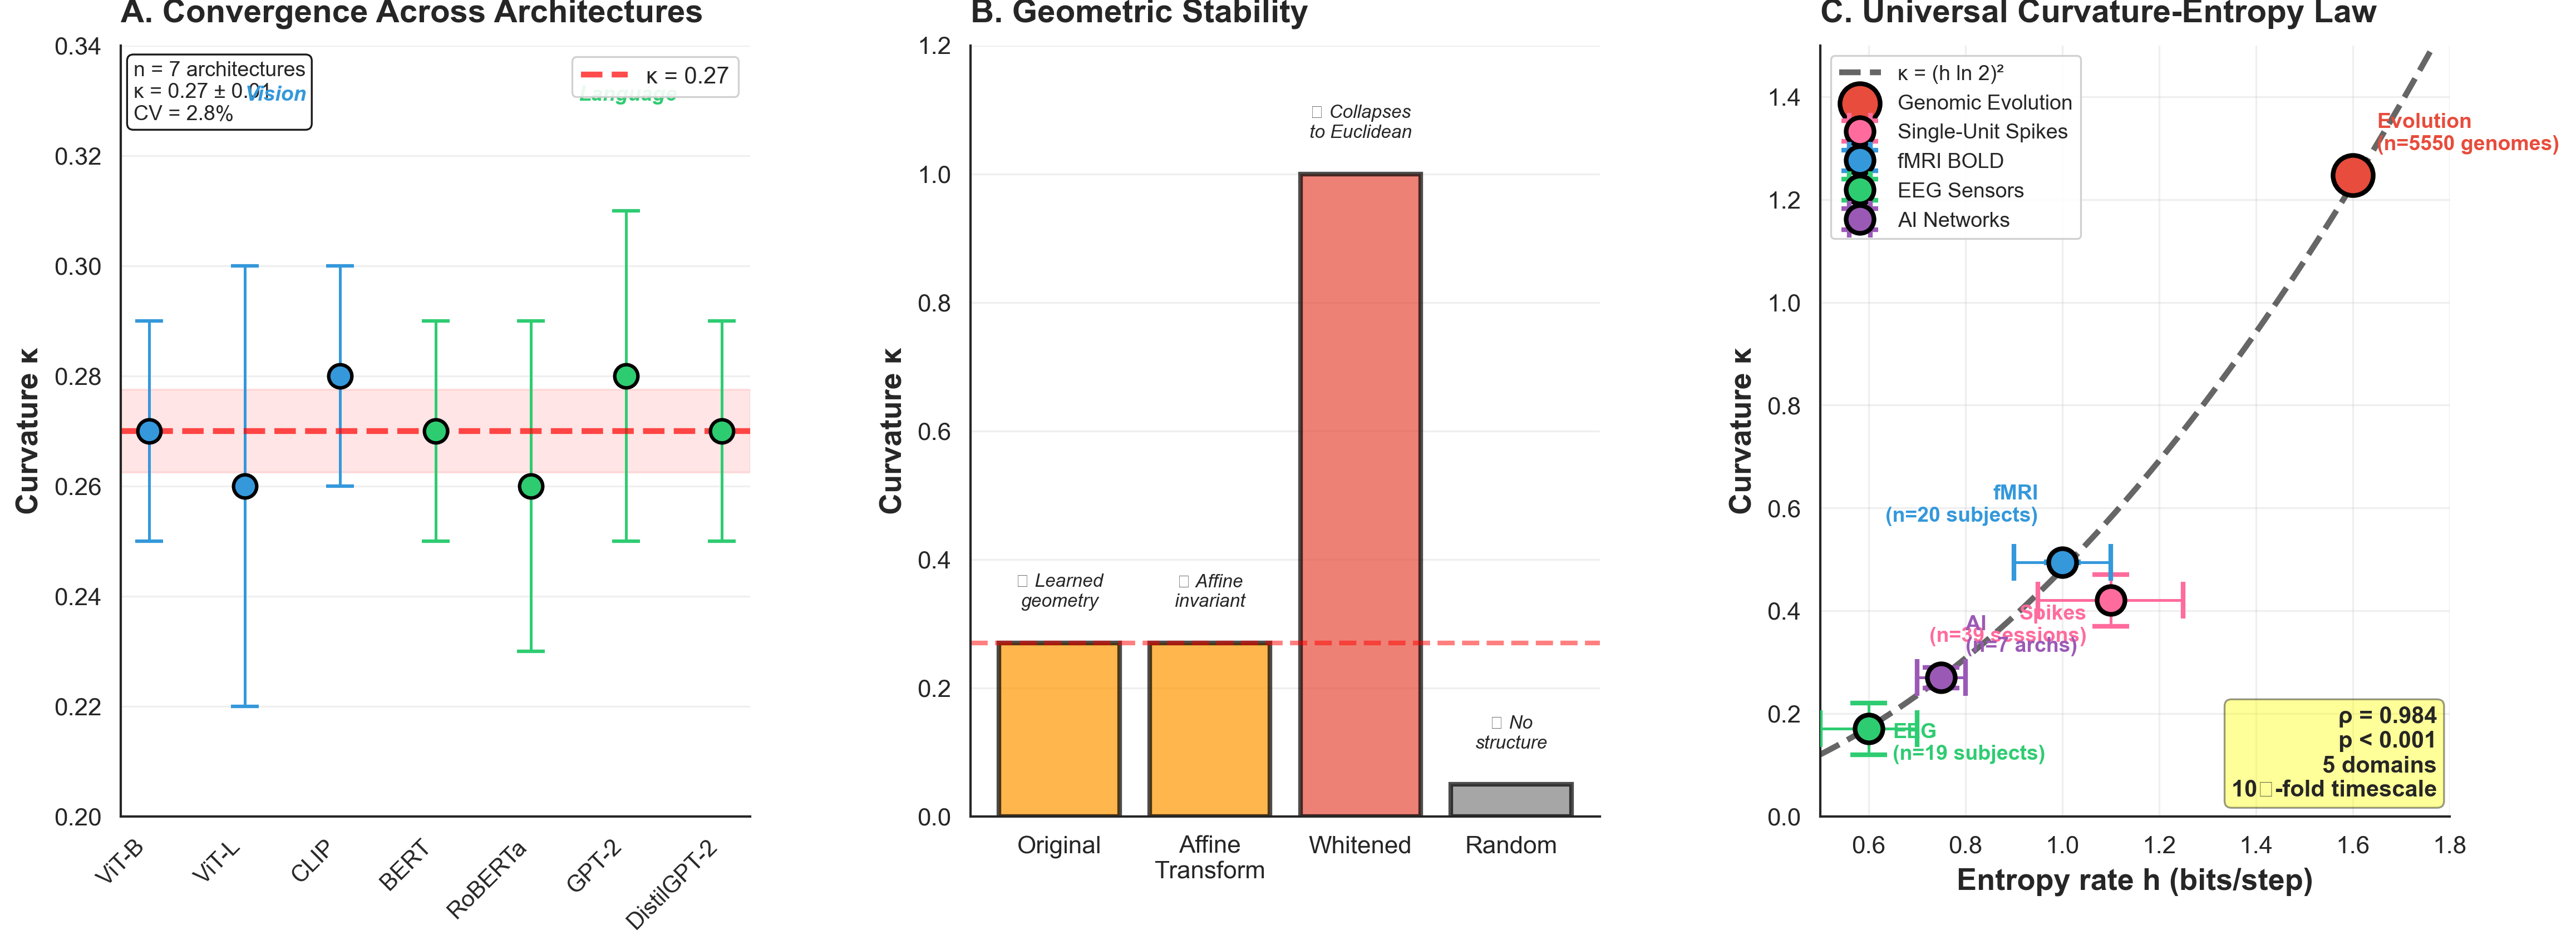
\includegraphics[width=\columnwidth]{figures/fig3_ai.png}
  \caption{AI validation and the universal curvature-entropy
    law.
    \textbf{(A)}~Seven architectures converge to
    $\kappa\approx0.27$ (CV~$=2.8\%$).
    \textbf{(B)}~Curvature collapses under whitening
    (destroys covariance structure) but is invariant to
    affine transforms, confirming the representation
    principle.
    \textbf{(C)}~$\kappa$ vs.\ $h$ across five domains
    falls on the zero-parameter curve
    $\kappa=(h\ln 2)^2$ ($\rho=0.984$, $p<0.001$);
    biological systems (filled circles) cluster above
    AI (open circle). Note: four of five entropy rates
    are back-solved (see Limitations).}
  \label{fig:ai}
\end{figure}

%% ===========================================================================
%% 5. DISCUSSION
%% ===========================================================================
\section{Discussion: Implications for Machine
Consciousness}\label{sec:discussion}

\subsection{Curvature as Second-Order Perception}

The curvature $\kappa$ is not a first-order property of
neural activity (firing rates, spectral power,
activation magnitudes) but a \emph{second-order}
geometric property of the interaction structure
among units.
It measures how the manifold of covariance
relationships curves---the geometry of how things
relate, not what they individually represent.

This distinction maps directly onto a structural
requirement shared by leading consciousness theories.
IIT requires that conscious systems exhibit
irreducible cause-effect structure---a property of the
\emph{relations} among elements, not of elements
themselves~\citep{tononi2004}.
GWT requires a shared workspace mediating interactions
among specialized modules~\citep{baars2005}.
The ``real problem'' approach emphasizes measurable
signatures of integration~\citep{seth2022}.
In all three frameworks, consciousness is
fundamentally about \emph{how parts interact}, not
what any part individually does.

The representation principle confirmed in
Table~\ref{tab:metric} makes this concrete:
the same GPT-2 activations, measured with metrics
sensitive only to marginal statistics (cosine, $L_2$),
yield negligible or negative curvature.
The geometric signature appears \emph{only} when we
measure interaction structure on SPD covariance
manifolds.
This suggests that any programme seeking to measure
consciousness in machines must use observables
sensitive to second-order interaction geometry, not
first-order activation statistics.

\subsection{Why the Geometric Gap Matters}

The finding that biological neural systems
($\kappa=0.4$--$0.5$) and current AI
($\kappa\approx0.27$) occupy distinct geometric
regimes has three implications.

First, it provides \emph{quantitative engineering
coordinates}.
If consciousness requires operation in the
biological $\kappa$ regime, we can now measure
progress toward consciousness-capable architectures
rather than relying on behavioral proxies.
Systems approaching biological $\kappa$ values
warrant investigation for consciousness-related
phenomena.

Second, the gap has a physical interpretation via the
state equation: biological systems explore at
$h\approx1.0$ bits/step while AI operates at
$h\approx0.75$.
This difference likely reflects the stochastic,
recurrent, embodied nature of biological computation
versus the directed, feedforward optimization of
gradient descent.
The 2.1\% layer-wise variation in GPT-2 suggests
current architectures are \emph{locked} at their
fixed point, potentially lacking the dynamic range
that biological systems exhibit.

Third, the gap is \emph{metric-specific}: it exists
only in SPD covariance geometry.
Analyses using cosine or Euclidean metrics on raw
representations would detect no difference between
neural and AI systems, explaining why prior work has
not identified this signature.

\subsection{Equilibrium vs.\ Dynamic Maintenance}

A crucial distinction for consciousness is between
systems that \emph{are} at equilibrium and systems that
\emph{actively maintain} equilibrium.
Both satisfy the state equation at any given
measurement, but only the latter exhibits the
dynamic properties that consciousness theories
typically require.

The field equation (Eq.~\ref{eq:master}) provides the
formal apparatus to distinguish them.
At equilibrium, $\dot{\kappa}=0$ and
$\kappa=\kappa^*=B/A$.
But $B(t)$ itself may be constant (passive
equilibrium) or dynamically regulated
(active maintenance).
The Lyapunov function (Eq.~\ref{eq:lyapunov}) proves
that perturbations from $\kappa^*$ decay exponentially
with timescale $\tau\sim A^{-1}$---but measuring
this relaxation requires \emph{perturbation
experiments}, not merely observational studies.

We conjecture that \emph{conscious systems actively
maintain $\kappa^*$ through ongoing regulation of
$B(t)$}, while merely hierarchical systems
(e.g., a pre-trained frozen network at inference)
sit passively at their fixed point.
This is empirically distinguishable: perturb the
system (e.g., targeted inactivation, fine-tuning
from modified initializations, anaesthetic
titration) and measure $\kappa(t)$ relaxation
dynamics.
Active maintenance predicts rapid restoration of
$\kappa^*$ with characteristic timescale $\tau$;
passive equilibrium predicts no such relaxation.

\subsection{Connection to Consciousness Theories}

\paragraph{Integrated Information Theory.}
Our geometric $\Phi_G$ (Eq.~\ref{eq:phi_g}) proposes a
computable surrogate, though its relationship to
Tononi's $\Phi$ remains conjectural.
While Tononi's $\Phi$ requires exponential-time
computation over all possible partitions, $\Phi_G$
is polynomial-time: $N_\mathrm{eff}$ from the
eigenspectrum, $C$ from the minimum information
partition rate, and $h$ from $\kappa$ via
Eq.~\eqref{eq:derive}.
$\Phi_G$ exhibits an inverted-U profile with respect
to $\kappa$: it is low both when the system is
incoherent (high $\kappa$, many modes but weak
integration) and when it is rigid (low $\kappa$, strong
integration but few modes).
The peak in the biological regime ($\kappa\approx0.5$)
is consistent with the IIT prediction that consciousness
correlates with maximum information
integration~\citep{tononi2004}.

\paragraph{Global Workspace Theory.}
The universality of $n=2$ across systems suggests a
binary branching architecture consistent with
broadcast-vs.-local processing topology.
High-$\kappa$ states (creative exploration)
correspond to divergent broadcasting; low-$\kappa$
states (absorption) to convergent local processing.
The EO/EC shift is consistent: closing eyes reduces
broadcast demands ($\downarrow J$), lowering
$\kappa^*$~\citep{baars2005}.

\paragraph{Predictive Processing.}
Curvature modulates the exploration-exploitation
tradeoff in prediction error minimization.
The $B(t)$ force balance
($\beta\langle J\rangle-\delta\langle\Phi\rangle$) can
be read as the tension between prediction
\emph{errors} (novelty, driving $\kappa$ up) and
prediction \emph{accuracy} (coherence, driving
$\kappa$ down)---precisely the free energy principle's
core dynamic.

\subsection{A Research Programme: Perturbation
Experiments}

We propose three concrete experiments to distinguish
active $\kappa$-maintenance from passive equilibrium:

\begin{enumerate}[nosep,leftmargin=*]
  \item \textbf{Graded anaesthesia.}
    Measure $\kappa(t)$ in EEG/fMRI during propofol
    titration.
    Prediction: $\kappa$ decreases monotonically with
    anaesthetic depth; the transition to unconsciousness
    corresponds to loss of $\kappa$-restoration dynamics
    (field equation Eq.~\ref{eq:master} loses its
    restoring term as coherence dominates).
  \item \textbf{AI layer ablation.}
    Surgically modify GPT-2 intermediate representations
    and measure $\kappa$ recovery during continued
    inference.
    Prediction: the frozen network cannot restore
    $\kappa$ (passive), while a network with ongoing
    learning dynamics can (active).
    Relaxation timescale $\tau$ provides a quantitative
    consciousness-relevant metric.
  \item \textbf{Cross-architecture comparison.}
    Measure $\kappa$ in recurrent networks (LSTM, state-space models) vs.\ feedforward transformers during
    active inference.
    Prediction: recurrent architectures with persistent
    state may exhibit faster $\kappa$ relaxation,
    closer to biological timescales.
\end{enumerate}

\subsection{Falsifiable Predictions}

The framework specifies conditions for falsification:
\begin{enumerate}[nosep,leftmargin=*]
  \item Independently measured entropy rates fail to
    predict curvatures within error bounds.
  \item Hierarchical systems consistently back-solve
    to $n\neq 2\pm 0.1$.
  \item Euclidean embeddings outperform hyperbolic at
    matched capacity ($\Delta\mathrm{AIC}<-10$).
  \item $\kappa$ varies by more than 15\% under
    temporal coarse-graining (RG breakdown).
  \item The state equation $h=(n{-}1)\sqrt{\kappa}/\ln 2$
    is violated with significance $p<0.01$.
\end{enumerate}
Unlike flexible frameworks adjusting to fit
observations, these create clear failure conditions.

\subsection{Limitations}

We acknowledge several limitations.
First, neural effect sizes are small
($\Delta\kappa=+0.015$ for single-unit, $+0.011$ for
EEG), requiring large datasets and careful null
construction.
Second, four of five entropy rates are back-solved
from $\kappa$, creating an inherently circular fit for
those domains.
The phylogenetic tree validation
(Section~\ref{sec:results}) provides one independent
check, but the remaining four domains lack independent
$h$ measurements.
Until these are obtained, the cross-domain
$\rho=0.984$ overstates the strength of evidence.
Third, the universal back-solved dimension $n=2$ may
partly reflect the measurement method: triangle-excess
curvature is defined on two-dimensional geodesic
sections, so a bias toward $n=2$ cannot be ruled out
without independent estimation of the embedding
dimension (e.g.\ via intrinsic-dimension estimators
applied to the same manifolds).
Fourth, all measurements are observational---the
perturbation experiments proposed above have not yet
been conducted.
Fifth, the field equations
(Eq.~\ref{eq:metric_flow}--\ref{eq:info_flow}) are
modelled under a constant-curvature ansatz that may
oversimplify rich neural dynamics.
Sixth, the EEG results are marginal, and replication
with higher-density arrays is needed.
Seventh, $\Phi_G$ is a conjecture, not a validated
measure of integrated information; its relationship
to Tononi's $\Phi$ remains undemonstrated.
Finally, we emphasise that $\kappa$ provides
\emph{necessary but not sufficient} conditions: the
state equation does not resolve the hard problem of
consciousness.

%% ===========================================================================
%% 6. CONCLUSION
%% ===========================================================================
\section{Conclusion}\label{sec:conclusion}

We have presented a geometric framework for measuring
hierarchical computation that provides substrate-independent
coordinates relevant to machine consciousness.
The zero-parameter state equation
$\kappa=(h\ln 2/(n{-}1))^2$ fits five domains
($\rho=0.984$), though four of five entropy rates are
back-solved (see Limitations); one independent check
(phylogenetic tree geometry) confirms the prediction
for evolution.
The state equation is machine-checked in Lean~4.
Field equations modelled on Perelman's Ricci-flow
entropy functional yield Lyapunov-stable curvature
dynamics, and the geometric integrated information
$\Phi_G$ offers a conjectured bridge to IIT in
computable form.

The empirically established geometric gap between
biological neural systems ($\kappa=0.4$--$0.5$) and
current AI ($\kappa\approx0.27$--$0.34$)---detectable
only on Riemannian covariance manifolds---provides
candidate quantitative coordinates for
consciousness-relevant information processing.
This gap is not a philosophical claim but a
measurable difference in interaction geometry.

For the machine consciousness community, we offer
three contributions:
(i)~a substrate-independent geometric invariant of
hierarchical computation that any theory must account
for;
(ii)~a dynamical theory (field equations +
Lyapunov stability) that distinguishes active
$\kappa$-maintenance from passive equilibrium---a
distinction potentially separating conscious from
merely computational systems; and
(iii)~concrete, falsifiable experimental predictions
that can adjudicate between these possibilities.

Whether the geometric gap between neural and artificial
systems reflects a fundamental barrier to machine
consciousness, or merely the current state of
architecture design, is an empirical question that
this framework makes answerable.

%% ===========================================================================
%% ACKNOWLEDGMENTS
%% ===========================================================================
\section*{Acknowledgments}

We thank the contributors to the Steinmetz Neuropixels
dataset, the ABIDE consortium, and PhysioNet.
Computational resources were provided by Sentry Bio,
Inc.

%% ===========================================================================
%% REFERENCES
%% ===========================================================================
\bibliographystyle{aaai}
\bibliography{references}

\end{document}
